\documentclass{article}
\usepackage[T1]{fontenc}
\usepackage{graphicx}
\graphicspath{ {./Images/} }

\title{Interfejsy, które utrudniają nam życie}
\author{Dominik Budzki}

\begin{document}
\maketitle

\section{PKP}
Pociągi to jeden z najpopularniejszych środków transportu w polsce,
dlatego ważnym jest aby cały system związany z tym środkiem lokomocyjnym działał sprawnie i nie sprawial problemów żadnej grupie społecznej.
W tych czasach powszechny dostęp do sieci internetowej sprawił iż PKP\footnote{Polskie Koleje Państwowe} musiały pozwolić Polakom na zakup biletów przez internet.
Przejdźmy więc proces zakupu biletu. Wyszukujemy w google stronę z rozkładem jazdy, znajdujemy połączenie które nas interesuje.
Klikamy "Zakup bilet" zostajemy przeniesieni na strone przewoźnika PKP i taki interfejs ukazuje się naszym oczom

\begin{center}
    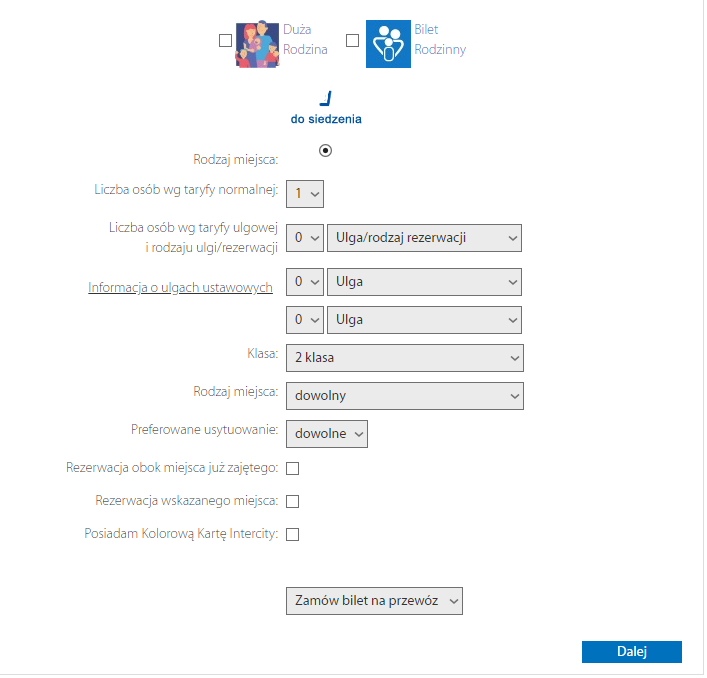
\includegraphics[scale=0.50]{Kupowanie-biletu.PNG}
\end{center}

\newpage
Pomijając miernej jakości warstwe graficzną, użytkownika zastanawia rubryka "Rodzaj miejsca" w której nie możemy nic wybrać (Po co ona w takim razie jest?).
Podczas wybierania kilku biletów z różnymi ulgami użytkownika może zastanawiać fakt czemu w jednym polu jest napis "Ulga/rodzaj rezerwacji" a w innym jest tylko "Ulga".
Interfejs ten wprowadza niepotrzebne zamieszanie zwłaszcza wśród osób niedoświadczonych w świecie komputerowym.
Największą ujmą jest tak naprawdę brak wyboru miejsca bezpośrednio. Taki wybór ma miejsce w zwykłych kinach, czemu nie może takiej opcji być w państwowych pociągach?
Bilet jest nam losowany, co więcej, gdy już zaznaczymy odpowiednie rubryki i klikniemy "Dalej" trafimy na taki obraz:

\begin{center}
    \includegraphics[scale=0.50]{informacje o bilecie.PNG}
\end{center}

Informacja jakie miejsce dostaliśmy pojawi nam się dopiero po kliknięciu opcji "Wybierz", co prowadzi do bardzo nieprzyjemnych sytuacji, gdyż osoba nie zaznajomiona z tym systemem
może pomyśleć, że musi zapłacić za bilet po kliknięciu a nawet nie wie jakie miejsce dostała. Wprowadza to niepotrzebny chaos przy kupowaniu zwykłego biletu na pociąg.

\newpage
\section{Toyota Celica}
Gdy kupowałem swoje auto dwa lata temu, uważałem że opcja podgrzewania siedzeń jest dużym plusem. Coś co miało uprzyjemnić podróż autem w zime, potrafi też niestety uprzykrzyć życie w lato.
Otóż przycisk do włączenia tego podgrzewania znajduje się jak widać na załączonym zdjęciu na podłokietniku. 

\begin{center}
    
\includegraphics[scale=0.07]{Celica1.jpg}
    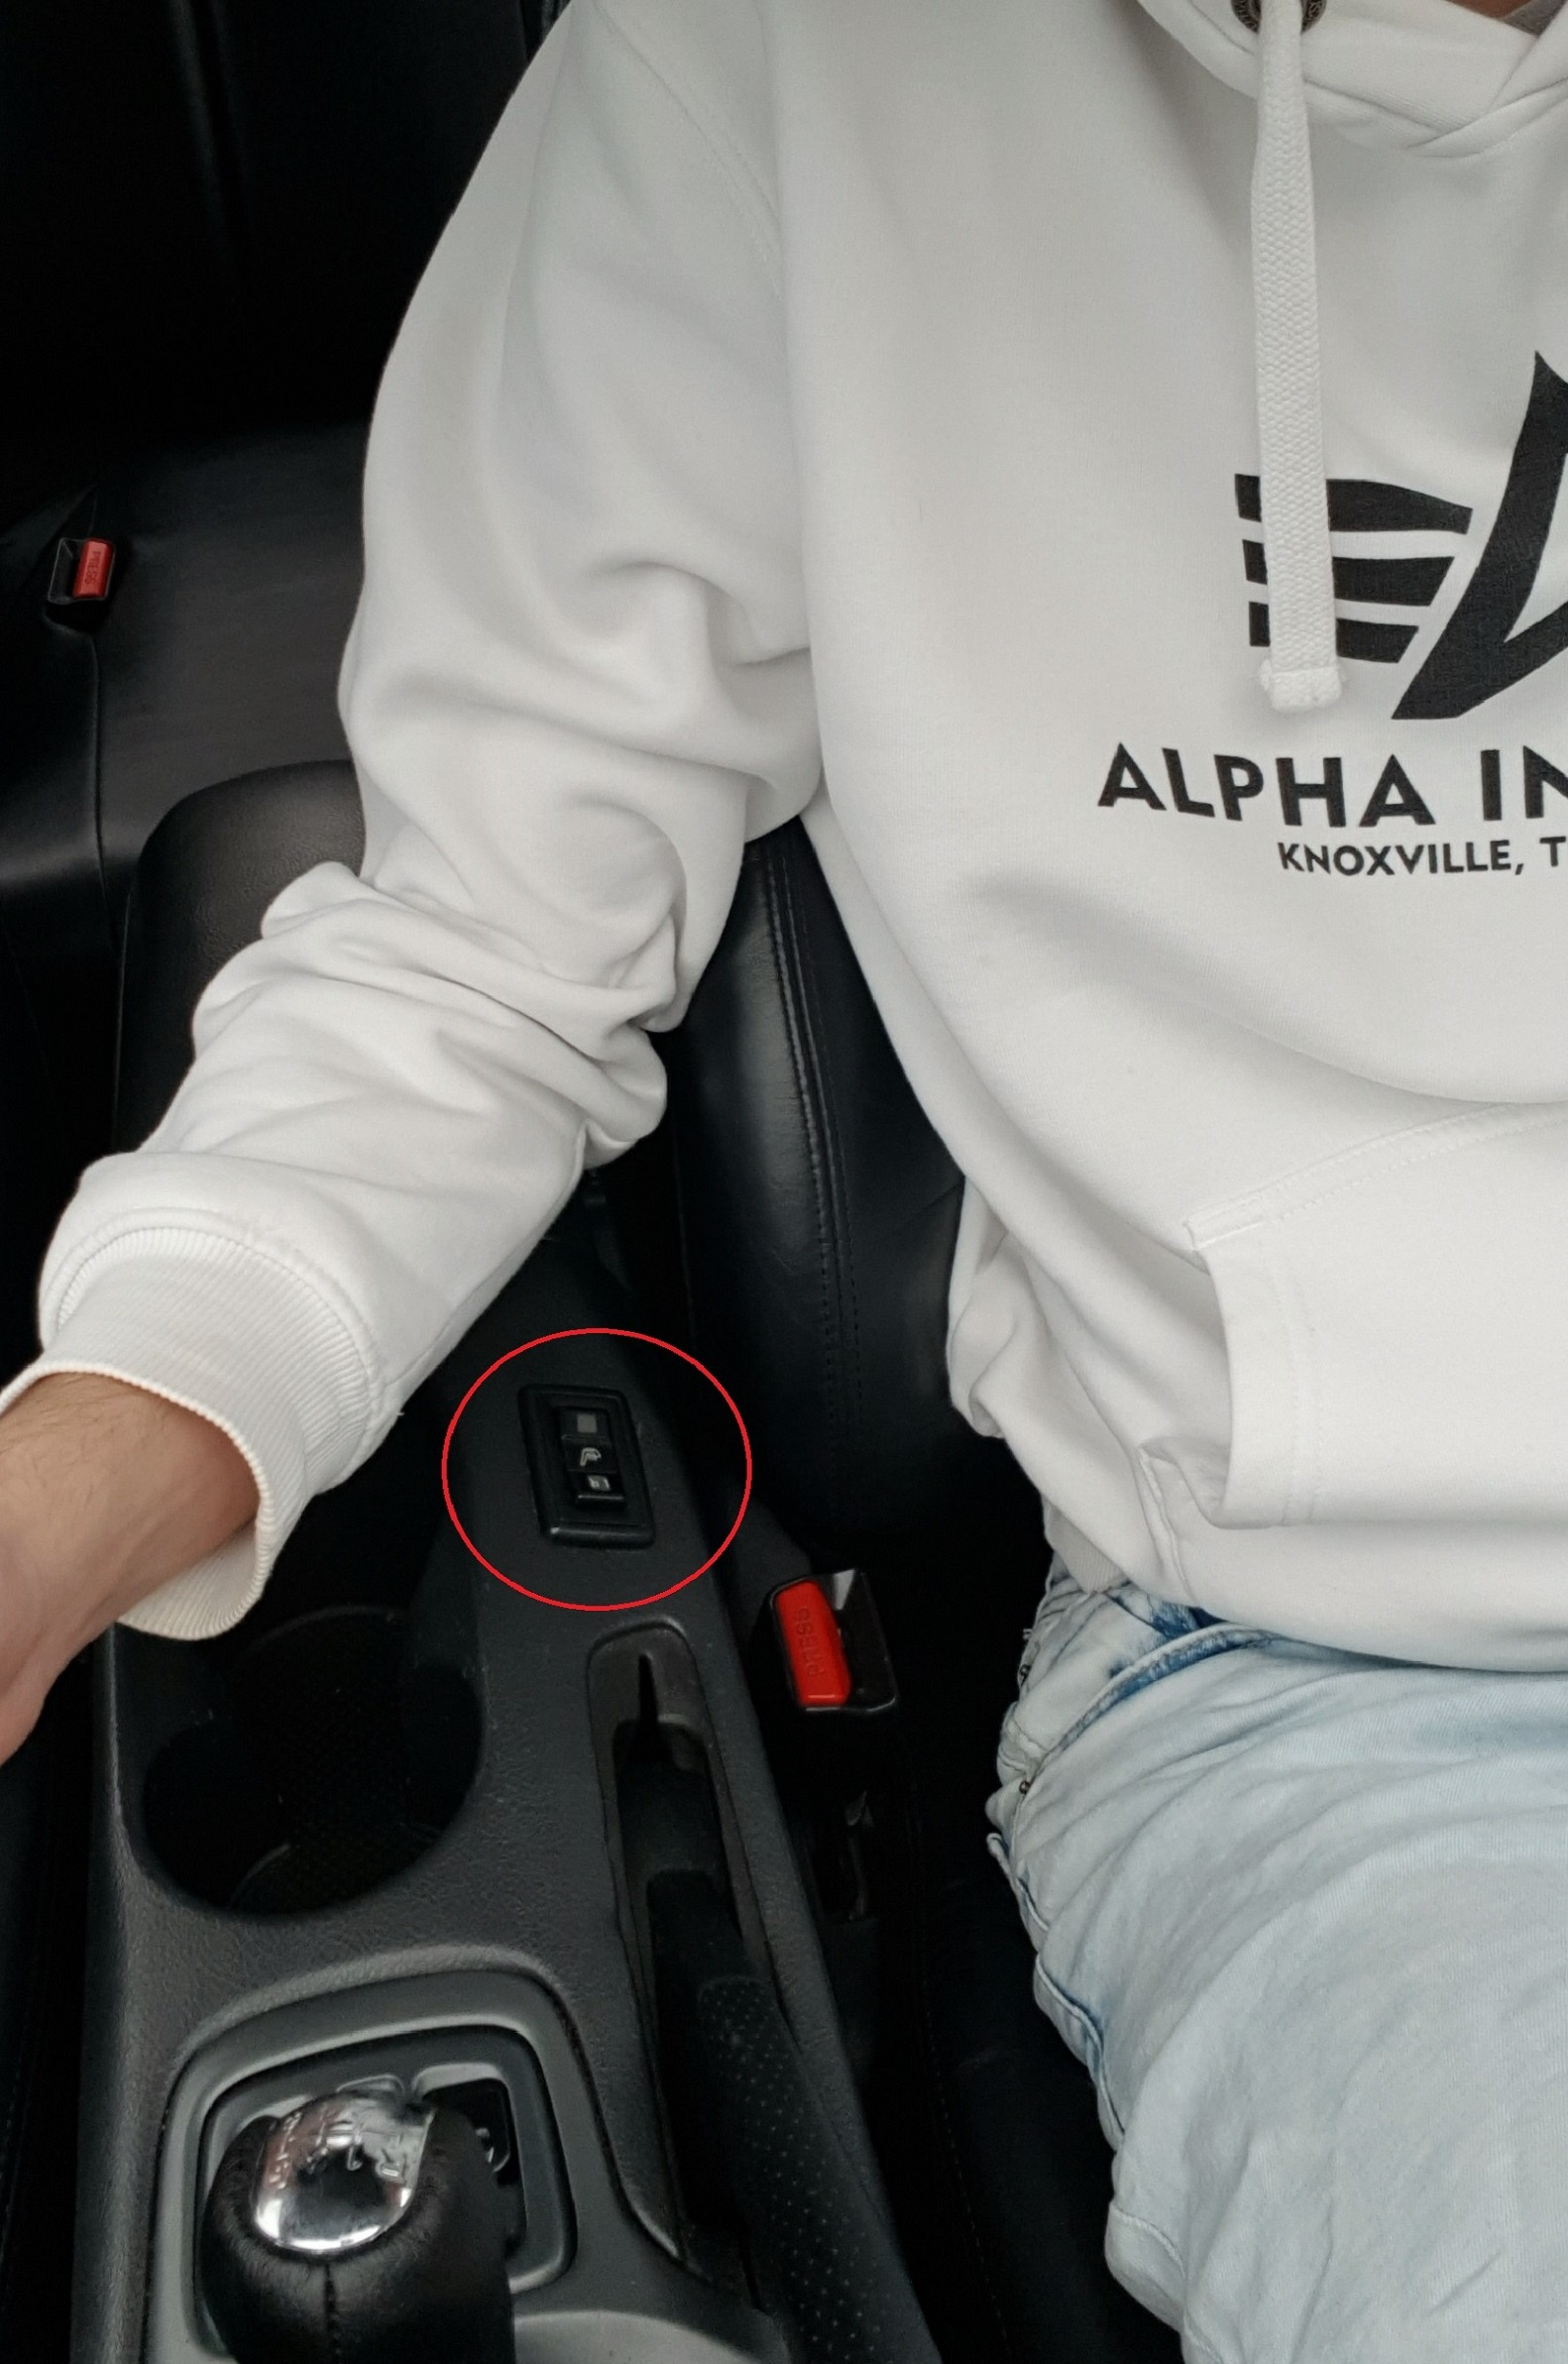
\includegraphics[scale=0.07]{Celica2.jpg}
\end{center}

Oczywiście można jeździć trzymając obie ręce na kierownicy, ale podczas jazdy w mieście gdzie musimy często
zmieniać biegi o wiele wygodniej jest trzymać łokieć właśnie w tym miejscu. Pare razy zdarzyło mi się niechcący włączyć podgrzewanie co w gorące lato prowadzi do dużego dyskomfortu. Autor mógł umieścić ten przycisk np.
przy przyciskach dotyczących klimatyzacji

\newpage
\section{Zapisywanie kontaktów w systemie Android}
Czasem bywa tak, że zadzwoni do nas nieznany numer, po czym okazuje się że jest to ktoś kogo znamy. Po udanej rozmowie chcemy zapisać ten numer w naszych kontaktach. Niestety Android w telefonie Samsung S8 w zakładce
"Ostatnie" nie ma zaimplementowanej funkcji zapisania numeru. Interfejs zmusza nas do wpisania tego numeru w klawiaturze i dopiero z tej pozycji zapisać numer, albo wymaga od nas żeby utworzyc nowy kontakt i 
tam wpisać numer. Jest to wielka niedogodność, która potrafi zdenerwować użytkownika.

\begin{center}
    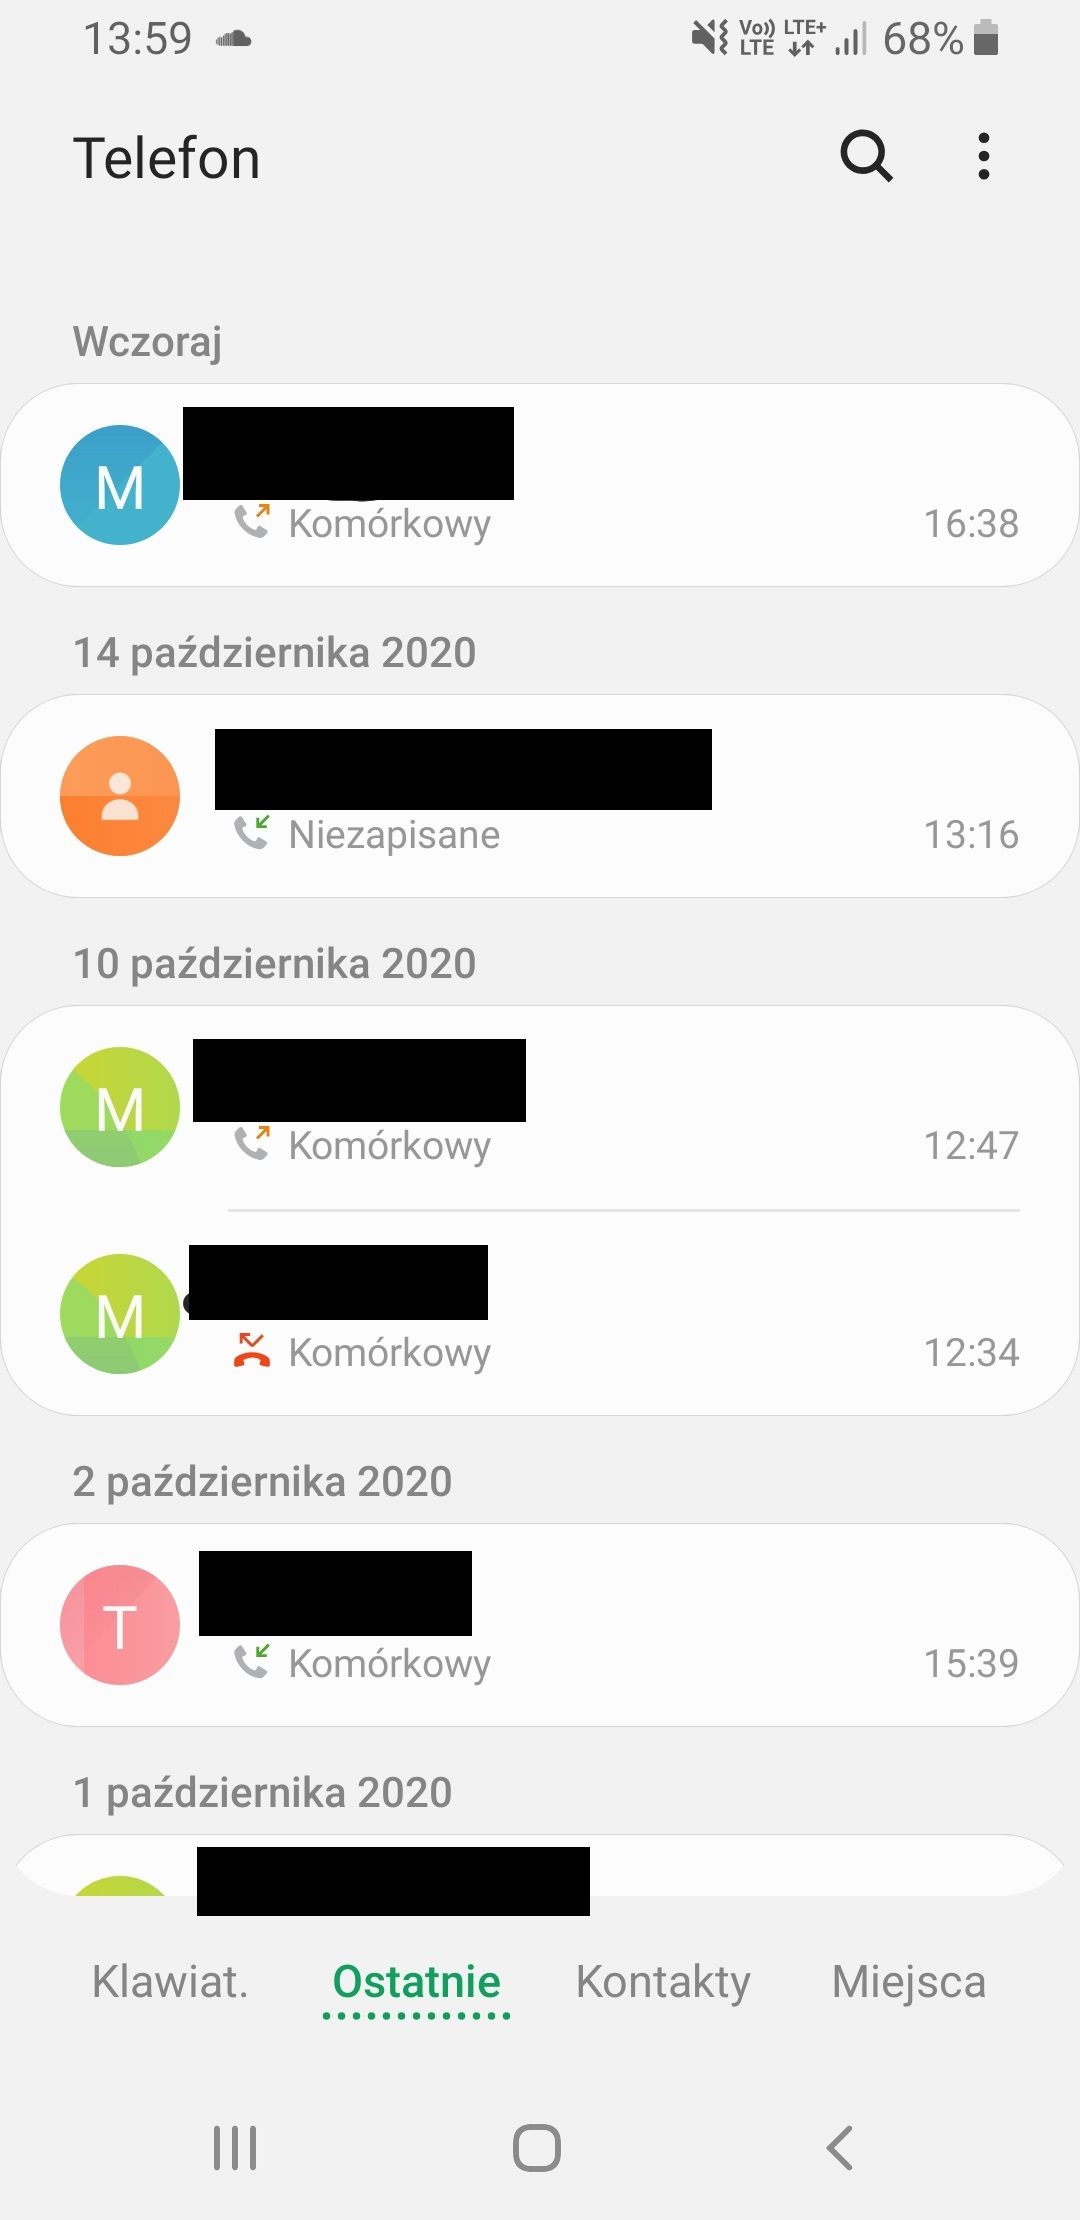
\includegraphics[scale=0.15]{Kontakty.jpg}
\end{center}


\end{document}